\documentclass{article}

%This file contains all packages and relevant definitions coming with them
%To use it add %This file contains all packages and relevant definitions coming with them
%To use it add %This file contains all packages and relevant definitions coming with them
%To use it add \input{../HEADERFILES_FOR_LATEX/PACKAGES} to the head of your file

%----------------------------------------------------------------------------------------------
%Typesetting
%----------------------------------------------------------------------------------------------
\usepackage[utf8]{inputenc} %To allow typesetting öäü

%----------------------------------------------------------------------------------------------
%Typesetting code
%----------------------------------------------------------------------------------------------
\usepackage{listings} %To allow nice typesetting of code

%Usage:
%Definition of all parameters defining the appearance of your code
%\lstset{ 
%	language=Matlab,% choose the language of the code
%	basicstyle=10pt,% the size of the fonts that are used for the code
%	numbers=left,% where to put the line-numbers
%	numberstyle=\footnotesize,% the size of the fonts that are used for the line-numbers
%	stepnumber=1,% the step between two line-numbers. If it's 1 each line will be numbered
%	numbersep=5pt,% how far the line-numbers are from the code
%	backgroundcolor=\color{SilverP},% choose the background color. You must add \usepackage{color}
%	showspaces=false,% show spaces adding particular underscores
%	showstringspaces=false,% underline spaces within strings
%	showtabs=false,% show tabs within strings adding particular underscores
% 	frame=single,% adds a frame around the code
% 	tabsize=2,% sets default tabsize to 2 spaces
% 	captionpos=t,% sets the caption-position to top
%	breaklines=true,% sets automatic line breaking
%	breakatwhitespace=false,% sets if automatic breaks should only happen at whitespace
%	escapeinside={\%*}{*)}% if you want to add a comment within your code
%}
%How to use it inside your document:
%\lstlistoflistings % To list all listings
%
%To input a whole file
%\lstinputlisting[language=Matlab,caption = Main file, label = lst:MainFile]{Code/LDC.m}
%
%To input some lines of code
%\begin{lstlisting
%#include <iostream>
%\end{lstlisting}


%----------------------------------------------------------------------------------------------
%Maths
%----------------------------------------------------------------------------------------------
\usepackage{amsmath} %Basic math package
\usepackage{amssymb} %Special symbols
\usepackage{siunitx} %Nice typesetting of numbers with units
%Usage:
%Use in math mode!
%For a unit without a number: \si{\kilo\gram\per\second}
%For a number with a unit: \SI{10e-12}{\nano\meter\per\second\squared}

%----------------------------------------------------------------------------------------------
%Formating
%----------------------------------------------------------------------------------------------

\usepackage[pdf]{graphviz}%Allows plotting graphs. Requires graphviz.
%example: 
%\digraph[scale=0.5]{abc}{rankdir=LR; a->b->c 
%a [label=<foo<SUP>bar</SUP>>];}

\usepackage{graphicx} %Placing of pictures
%Usage:
%\includegraphics[width=\linewidth]{<Name of picture in pictures without filetype extension/>}
\graphicspath{ {pictures/} } %Allows to include pictures with only their name instead of the path

\usepackage{multicol} %Dividing the page into multiple columns
%Usage:
%\begin{multicols}{<number of colums>}<your content>\end{multicols}

\usepackage{wrapfig} %Allows to wrap text around figures
%Usage:
%\begin{wrapfigure}[<Number of narrow lines>]{<placement>}[<overhang in pt> pt]
% <some figure>
%\end{wrapfigure}

\usepackage[table]{xcolor} %Allows the use of an array of colors
%Option: table Load the colortbl package, in order to use the tools for coloring rows, columns, and cells within tables
%Usage:
%Change textcolor: \textcolor{<color>}{<text>}
%Make a colorbox: \fcolorbox{<box color>{<background color>} 

\usepackage{booktabs} %Allows making nicer tables
%Usage:
%Make a nice horizontal midrule: \midrule

\usepackage{float} %An improved environment for floating figures

\usepackage{fancyhdr} %Allows manipulation of headers and footers

\usepackage{blindtext} %Allows generation of blind text
%Usage:
%One paragraph of lorem ipsum: \blindtext
%A certain number of paragraphs: \Blindtext[X][Y]
%where X is the number of paragraphs and Y is the number of pangrams

\usepackage{enumitem} %Allows configure enumerations and such
%Usage:
%\begin{itemize}[leftmargin=*,noitemsep,topsep=0pt]
%\item <content>
%\end{itemize}
%This examples leaves away the margin on the left, sets the item seperation to zero and leaves away the
%white space generated above an enumeration/itemization

\usepackage{longtable, tabularx} %Allows the introduction of special columntypes for tabular environments
\newcolumntype{L}[1]{>{\raggedright\arraybackslash}p{#1}} % raggedleft column 
\newcolumntype{C}[1]{>{\centering\arraybackslash}p{#1}} % centered column
\newcolumntype{R}[1]{>{\raggedleft\arraybackslash}p{#1}} % raggedright column
%Usage:
%\begin{tabular}{L{2cm}|L{2cm}|L{2cm}|L{3cm}|L{3cm}}
%<content>
%\end{tabular}

\usepackage{lscape} %Allows the use of single landscape pages within a document in portrait orientation
%Usage:
%\begin{landscape}
%<content>
%\end{landscape}

\usepackage[hidelinks]{hyperref} %allows for clickable references, doesn't colour the links

\usepackage{pgfplots} %allows including specially exported .svg-figures
%You want nice vector-graphics in your document that even have latex-fonts? Ask Gianni.
%Also allows doing tikzpictures!
%Usage:
%\begin{tikzpicture}
%\begin{axis}[
%    axis lines = left,
%    xlabel = {$h$ in $\si{mm}$},
%    ylabel = {$C_{D\Theta,corrected}$},
%]
%\addplot [
%    domain=5:45, 
%    samples=100, 
%    color=MyPomegranate,
%]
%{1.17*(1-0.25*8.93/x)};
%\end{axis}
%\end{tikzpicture}}


%\usepackage[ %Allows importing your bibliography from another file
%backend = biber,
%style = ieee,
%natbib = true,
%url = true,
%doi = false,
%eprint = false,
%]{biblatex}
%Usage:
%\addbibresource{<Absolute/Path/To/Your/.bib/file.bib>}
%\printbiblbiography %Add this line where you'd like to print your bibliography

%----------------------------------------------------------------------------------------------
%LaTeX workarounds
%----------------------------------------------------------------------------------------------

\usepackage{xparse} %Allows to define new environments with arguments passed to the \end{env}-part
%Consider reading: https://tex.stackexchange.com/questions/17036/why-cant-the-end-code-of-an-environment-contain-an-argument
%Usage:
%\NewDocumentEnvironment{foo}{m}
%  {some code #1}
%  {some code #1}

%----------------------------------------------------------------------------------------------
%Additions AIAA
%----------------------------------------------------------------------------------------------
\usepackage[version=4]{mhchem} %Allows using signs for chemical equations and other fancy stuff
\usepackage{pdfpages} %To add pdf files
\usepackage{appendix} %For appendix typesettings to the head of your file

%----------------------------------------------------------------------------------------------
%Typesetting
%----------------------------------------------------------------------------------------------
\usepackage[utf8]{inputenc} %To allow typesetting öäü

%----------------------------------------------------------------------------------------------
%Typesetting code
%----------------------------------------------------------------------------------------------
\usepackage{listings} %To allow nice typesetting of code

%Usage:
%Definition of all parameters defining the appearance of your code
%\lstset{ 
%	language=Matlab,% choose the language of the code
%	basicstyle=10pt,% the size of the fonts that are used for the code
%	numbers=left,% where to put the line-numbers
%	numberstyle=\footnotesize,% the size of the fonts that are used for the line-numbers
%	stepnumber=1,% the step between two line-numbers. If it's 1 each line will be numbered
%	numbersep=5pt,% how far the line-numbers are from the code
%	backgroundcolor=\color{SilverP},% choose the background color. You must add \usepackage{color}
%	showspaces=false,% show spaces adding particular underscores
%	showstringspaces=false,% underline spaces within strings
%	showtabs=false,% show tabs within strings adding particular underscores
% 	frame=single,% adds a frame around the code
% 	tabsize=2,% sets default tabsize to 2 spaces
% 	captionpos=t,% sets the caption-position to top
%	breaklines=true,% sets automatic line breaking
%	breakatwhitespace=false,% sets if automatic breaks should only happen at whitespace
%	escapeinside={\%*}{*)}% if you want to add a comment within your code
%}
%How to use it inside your document:
%\lstlistoflistings % To list all listings
%
%To input a whole file
%\lstinputlisting[language=Matlab,caption = Main file, label = lst:MainFile]{Code/LDC.m}
%
%To input some lines of code
%\begin{lstlisting
%#include <iostream>
%\end{lstlisting}


%----------------------------------------------------------------------------------------------
%Maths
%----------------------------------------------------------------------------------------------
\usepackage{amsmath} %Basic math package
\usepackage{amssymb} %Special symbols
\usepackage{siunitx} %Nice typesetting of numbers with units
%Usage:
%Use in math mode!
%For a unit without a number: \si{\kilo\gram\per\second}
%For a number with a unit: \SI{10e-12}{\nano\meter\per\second\squared}

%----------------------------------------------------------------------------------------------
%Formating
%----------------------------------------------------------------------------------------------

\usepackage[pdf]{graphviz}%Allows plotting graphs. Requires graphviz.
%example: 
%\digraph[scale=0.5]{abc}{rankdir=LR; a->b->c 
%a [label=<foo<SUP>bar</SUP>>];}

\usepackage{graphicx} %Placing of pictures
%Usage:
%\includegraphics[width=\linewidth]{<Name of picture in pictures without filetype extension/>}
\graphicspath{ {pictures/} } %Allows to include pictures with only their name instead of the path

\usepackage{multicol} %Dividing the page into multiple columns
%Usage:
%\begin{multicols}{<number of colums>}<your content>\end{multicols}

\usepackage{wrapfig} %Allows to wrap text around figures
%Usage:
%\begin{wrapfigure}[<Number of narrow lines>]{<placement>}[<overhang in pt> pt]
% <some figure>
%\end{wrapfigure}

\usepackage[table]{xcolor} %Allows the use of an array of colors
%Option: table Load the colortbl package, in order to use the tools for coloring rows, columns, and cells within tables
%Usage:
%Change textcolor: \textcolor{<color>}{<text>}
%Make a colorbox: \fcolorbox{<box color>{<background color>} 

\usepackage{booktabs} %Allows making nicer tables
%Usage:
%Make a nice horizontal midrule: \midrule

\usepackage{float} %An improved environment for floating figures

\usepackage{fancyhdr} %Allows manipulation of headers and footers

\usepackage{blindtext} %Allows generation of blind text
%Usage:
%One paragraph of lorem ipsum: \blindtext
%A certain number of paragraphs: \Blindtext[X][Y]
%where X is the number of paragraphs and Y is the number of pangrams

\usepackage{enumitem} %Allows configure enumerations and such
%Usage:
%\begin{itemize}[leftmargin=*,noitemsep,topsep=0pt]
%\item <content>
%\end{itemize}
%This examples leaves away the margin on the left, sets the item seperation to zero and leaves away the
%white space generated above an enumeration/itemization

\usepackage{longtable, tabularx} %Allows the introduction of special columntypes for tabular environments
\newcolumntype{L}[1]{>{\raggedright\arraybackslash}p{#1}} % raggedleft column 
\newcolumntype{C}[1]{>{\centering\arraybackslash}p{#1}} % centered column
\newcolumntype{R}[1]{>{\raggedleft\arraybackslash}p{#1}} % raggedright column
%Usage:
%\begin{tabular}{L{2cm}|L{2cm}|L{2cm}|L{3cm}|L{3cm}}
%<content>
%\end{tabular}

\usepackage{lscape} %Allows the use of single landscape pages within a document in portrait orientation
%Usage:
%\begin{landscape}
%<content>
%\end{landscape}

\usepackage[hidelinks]{hyperref} %allows for clickable references, doesn't colour the links

\usepackage{pgfplots} %allows including specially exported .svg-figures
%You want nice vector-graphics in your document that even have latex-fonts? Ask Gianni.
%Also allows doing tikzpictures!
%Usage:
%\begin{tikzpicture}
%\begin{axis}[
%    axis lines = left,
%    xlabel = {$h$ in $\si{mm}$},
%    ylabel = {$C_{D\Theta,corrected}$},
%]
%\addplot [
%    domain=5:45, 
%    samples=100, 
%    color=MyPomegranate,
%]
%{1.17*(1-0.25*8.93/x)};
%\end{axis}
%\end{tikzpicture}}


%\usepackage[ %Allows importing your bibliography from another file
%backend = biber,
%style = ieee,
%natbib = true,
%url = true,
%doi = false,
%eprint = false,
%]{biblatex}
%Usage:
%\addbibresource{<Absolute/Path/To/Your/.bib/file.bib>}
%\printbiblbiography %Add this line where you'd like to print your bibliography

%----------------------------------------------------------------------------------------------
%LaTeX workarounds
%----------------------------------------------------------------------------------------------

\usepackage{xparse} %Allows to define new environments with arguments passed to the \end{env}-part
%Consider reading: https://tex.stackexchange.com/questions/17036/why-cant-the-end-code-of-an-environment-contain-an-argument
%Usage:
%\NewDocumentEnvironment{foo}{m}
%  {some code #1}
%  {some code #1}

%----------------------------------------------------------------------------------------------
%Additions AIAA
%----------------------------------------------------------------------------------------------
\usepackage[version=4]{mhchem} %Allows using signs for chemical equations and other fancy stuff
\usepackage{pdfpages} %To add pdf files
\usepackage{appendix} %For appendix typesettings to the head of your file

%----------------------------------------------------------------------------------------------
%Typesetting
%----------------------------------------------------------------------------------------------
\usepackage[utf8]{inputenc} %To allow typesetting öäü

%----------------------------------------------------------------------------------------------
%Typesetting code
%----------------------------------------------------------------------------------------------
\usepackage{listings} %To allow nice typesetting of code

%Usage:
%Definition of all parameters defining the appearance of your code
%\lstset{ 
%	language=Matlab,% choose the language of the code
%	basicstyle=10pt,% the size of the fonts that are used for the code
%	numbers=left,% where to put the line-numbers
%	numberstyle=\footnotesize,% the size of the fonts that are used for the line-numbers
%	stepnumber=1,% the step between two line-numbers. If it's 1 each line will be numbered
%	numbersep=5pt,% how far the line-numbers are from the code
%	backgroundcolor=\color{SilverP},% choose the background color. You must add \usepackage{color}
%	showspaces=false,% show spaces adding particular underscores
%	showstringspaces=false,% underline spaces within strings
%	showtabs=false,% show tabs within strings adding particular underscores
% 	frame=single,% adds a frame around the code
% 	tabsize=2,% sets default tabsize to 2 spaces
% 	captionpos=t,% sets the caption-position to top
%	breaklines=true,% sets automatic line breaking
%	breakatwhitespace=false,% sets if automatic breaks should only happen at whitespace
%	escapeinside={\%*}{*)}% if you want to add a comment within your code
%}
%How to use it inside your document:
%\lstlistoflistings % To list all listings
%
%To input a whole file
%\lstinputlisting[language=Matlab,caption = Main file, label = lst:MainFile]{Code/LDC.m}
%
%To input some lines of code
%\begin{lstlisting
%#include <iostream>
%\end{lstlisting}


%----------------------------------------------------------------------------------------------
%Maths
%----------------------------------------------------------------------------------------------
\usepackage{amsmath} %Basic math package
\usepackage{amssymb} %Special symbols
\usepackage{siunitx} %Nice typesetting of numbers with units
%Usage:
%Use in math mode!
%For a unit without a number: \si{\kilo\gram\per\second}
%For a number with a unit: \SI{10e-12}{\nano\meter\per\second\squared}

%----------------------------------------------------------------------------------------------
%Formating
%----------------------------------------------------------------------------------------------

\usepackage[pdf]{graphviz}%Allows plotting graphs. Requires graphviz.
%example: 
%\digraph[scale=0.5]{abc}{rankdir=LR; a->b->c 
%a [label=<foo<SUP>bar</SUP>>];}

\usepackage{graphicx} %Placing of pictures
%Usage:
%\includegraphics[width=\linewidth]{<Name of picture in pictures without filetype extension/>}
\graphicspath{ {pictures/} } %Allows to include pictures with only their name instead of the path

\usepackage{multicol} %Dividing the page into multiple columns
%Usage:
%\begin{multicols}{<number of colums>}<your content>\end{multicols}

\usepackage{wrapfig} %Allows to wrap text around figures
%Usage:
%\begin{wrapfigure}[<Number of narrow lines>]{<placement>}[<overhang in pt> pt]
% <some figure>
%\end{wrapfigure}

\usepackage[table]{xcolor} %Allows the use of an array of colors
%Option: table Load the colortbl package, in order to use the tools for coloring rows, columns, and cells within tables
%Usage:
%Change textcolor: \textcolor{<color>}{<text>}
%Make a colorbox: \fcolorbox{<box color>{<background color>} 

\usepackage{booktabs} %Allows making nicer tables
%Usage:
%Make a nice horizontal midrule: \midrule

\usepackage{float} %An improved environment for floating figures

\usepackage{fancyhdr} %Allows manipulation of headers and footers

\usepackage{blindtext} %Allows generation of blind text
%Usage:
%One paragraph of lorem ipsum: \blindtext
%A certain number of paragraphs: \Blindtext[X][Y]
%where X is the number of paragraphs and Y is the number of pangrams

\usepackage{enumitem} %Allows configure enumerations and such
%Usage:
%\begin{itemize}[leftmargin=*,noitemsep,topsep=0pt]
%\item <content>
%\end{itemize}
%This examples leaves away the margin on the left, sets the item seperation to zero and leaves away the
%white space generated above an enumeration/itemization

\usepackage{longtable, tabularx} %Allows the introduction of special columntypes for tabular environments
\newcolumntype{L}[1]{>{\raggedright\arraybackslash}p{#1}} % raggedleft column 
\newcolumntype{C}[1]{>{\centering\arraybackslash}p{#1}} % centered column
\newcolumntype{R}[1]{>{\raggedleft\arraybackslash}p{#1}} % raggedright column
%Usage:
%\begin{tabular}{L{2cm}|L{2cm}|L{2cm}|L{3cm}|L{3cm}}
%<content>
%\end{tabular}

\usepackage{lscape} %Allows the use of single landscape pages within a document in portrait orientation
%Usage:
%\begin{landscape}
%<content>
%\end{landscape}

\usepackage[hidelinks]{hyperref} %allows for clickable references, doesn't colour the links

\usepackage{pgfplots} %allows including specially exported .svg-figures
%You want nice vector-graphics in your document that even have latex-fonts? Ask Gianni.
%Also allows doing tikzpictures!
%Usage:
%\begin{tikzpicture}
%\begin{axis}[
%    axis lines = left,
%    xlabel = {$h$ in $\si{mm}$},
%    ylabel = {$C_{D\Theta,corrected}$},
%]
%\addplot [
%    domain=5:45, 
%    samples=100, 
%    color=MyPomegranate,
%]
%{1.17*(1-0.25*8.93/x)};
%\end{axis}
%\end{tikzpicture}}


%\usepackage[ %Allows importing your bibliography from another file
%backend = biber,
%style = ieee,
%natbib = true,
%url = true,
%doi = false,
%eprint = false,
%]{biblatex}
%Usage:
%\addbibresource{<Absolute/Path/To/Your/.bib/file.bib>}
%\printbiblbiography %Add this line where you'd like to print your bibliography

%----------------------------------------------------------------------------------------------
%LaTeX workarounds
%----------------------------------------------------------------------------------------------

\usepackage{xparse} %Allows to define new environments with arguments passed to the \end{env}-part
%Consider reading: https://tex.stackexchange.com/questions/17036/why-cant-the-end-code-of-an-environment-contain-an-argument
%Usage:
%\NewDocumentEnvironment{foo}{m}
%  {some code #1}
%  {some code #1}

%----------------------------------------------------------------------------------------------
%Additions AIAA
%----------------------------------------------------------------------------------------------
\usepackage[version=4]{mhchem} %Allows using signs for chemical equations and other fancy stuff
\usepackage{pdfpages} %To add pdf files
\usepackage{appendix} %For appendix typesettings
%This file contains all commands simplifying LaTeX text editing
%For each new command clearly document its dependencies (packages) and its use
%Adhere to the ordering by category!

%----------------------------------------------------------------------------------------------
%Maths
%----------------------------------------------------------------------------------------------
\renewcommand{\vec}[1]{\boldsymbol{#1}} %Notation of vectors
\newcommand{\vect}[1]{\dot{\boldsymbol{#1}}} %Notation of time derivative of a vector
\newcommand{\vectt}[1]{\ddot{\boldsymbol{#1}}} %Notation of the second time derivative of a vector
\newcommand{\vecd}[1]{\boldsymbol{#1'}} %Notation of the first derivative of a vector
\newcommand{\vecdd}[1]{\boldsymbol{#1''}} 
%In the following all vector definitions will be repeated with the inclusion of a prepended calligraphic letter to define the respective coordinate frame
\newcommand{\cvec}[2]{{}_\mathcal{#1}\boldsymbol{#2}} %Notation of vectors
\newcommand{\cvect}[2]{{}_\mathcal{#1}\dot{\boldsymbol{#2}}} %Notation of time derivative of a vector
\newcommand{\cvectt}[2]{{}_\mathcal{#1}\boldsymbol{\ddot{#2}}} %Notation of the second time derivative of a vector
\newcommand{\cvecd}[2]{{}_\mathcal{#1}\boldsymbol{#2'}} %Notation of the first derivative of a vector
\newcommand{\cvecdd}[2]{{}_\mathcal{#1}\boldsymbol{#2''}}

%Notation of rotation matrices
\newcommand{\rotmat}[2]{\boldsymbol{#1}_{\mathcal{#2}}}

%Notation of the second derivative of a vector
\newcommand{\tens}[1]{\underline{\underline{#1}}} %Notation of a tensor
\newcommand{\vprod}[2]{\vec{#1}\times\vec{#2}} %Vector product
\newcommand{\inRone}[1]{\in\mathbb{R}^{#1}} %in 1D set of real numbers
\newcommand{\inRtwo}[2]{\in\mathbb{R}^{#1 \times #2}} %in 2D set of real numbers
\newcommand{\inRthree}[3]{\in\mathbb{R}^{#1 \times #2 \times #3}} %in 3D set of real numbers
\newcommand{\ddt}{\frac{d}{dt}} %time derivative of
\newcommand{\onha}{\frac{1}{2}} %one half
\newcommand{\onth}{\frac{1}{3}} %one third
\newcommand{\onfo}{\frac{1}{4}} %one forth
\newcommand{\prob}[1]{\mathbb{P}(#1)} %Probability of some event
\newcommand{\expe}[1]{\mathbb{E}[#1]} %Expected value for some stochastic variable
\newcommand{\var}[1]{\text{Var}(#1)} %Variance of some stochastic variable
\newcommand{\cov}[1]{\text{Cov}(#1)} %Covariance of some stochastic variables
\newcommand{\corr}[1]{\text{Corr}(#1)} %Correlation of some stochastic variables
\newcommand{\sign}[1]{\text{sign}(#1)} %signum function
\newcommand{\sinc}{\text{sinc}} %sinc function
\newcommand{\diag}{\text{diag}} %diagonal matrix
\newcommand{\expnum}[2]{{#1}\cdot 10^{#2}} %exponential number

%----------------------------------------------------------------------------------------------
%Tables
%----------------------------------------------------------------------------------------------

\newcommand{\mc}[2]{\multicolumn{1}{#1}{#2}} %This command is a short for multicolumn
%Usage:
%Instead of \multicolumn{1}{<type>}{<content>}
%write \mc{<type>}{<content>}
%Usecase: When trying to remove vertical lines for only one line in your tabular environment
%multicolumn can come in handy.

%----------------------------------------------------------------------------------------------
% Formating
%----------------------------------------------------------------------------------------------

%Command for inserting [...] into a quote
\newcommand{\etcetera}{$[\ldots]\ $}

\newcommand{\sbs}[4]{\begin{minipage}[t!]{#1\linewidth}#3\end{minipage}\begin{minipage}[t!]{#2\linewidth}#4\end{minipage}} %Two minipages dividing the page in two scaled parts
%Usage:
%\sbs{<width of the left, for example 0.45>}{<width on the right, for example 0.45>}
%{
%<content on the left>
%}
%{
%<content on the right>
%}

\newcommand{\sbss}[2]{\sbs{0.45}{0.45}{#1}{#2}} %Two minipages dividing the page in two equal parts
%Usage:
%\sbss
%{
%<content on the left>
%}
%{
%<content on the right>
%}


\newcommand{\sbsss}[3]{\begin{minipage}[t!]{0.42\linewidth}#2\end{minipage}\hspace{#1 ex}\begin{minipage}[t!]{0.42\linewidth}#3\end{minipage}} %Two minipages dividing the page in two equal parts with some user-defined space in [ex] in between
%Usage:
%\sbsss{5}
%{
%<content on the left>
%}
%{
%<content on the right>
%}

%Easy notation of physical units
\newcommand{\siu}[1]{[\si{#1}]}

%----------------------------------------------------------------------------------------------
%Colors
%----------------------------------------------------------------------------------------------
\definecolor{pantone2128}{RGB}{152,182,228}
\definecolor{pantone2727}{RGB}{48,127,226}
\definecolor{pantone2728}{RGB}{0,71,187}
\definecolor{darkblue}{RGB}{0,35,156}
\definecolor{pantone2757}{RGB}{0,30,96}

%----------------------------------------------------------------------------------------------
%Macros
%----------------------------------------------------------------------------------------------

\newcommand{\statenotation}{
\section{Notation}
\begin{center}
\begin{tabular}{p{0.3\linewidth}p{0.3\linewidth}l}
Operator&Meaning&Example\\
\midrule
\textit{italic}&scalars&$m$\\
\textbf{bold letter}&Vector&$\vec{v}$\\
\textbf{bold capital}&Matrix&$\vec{C}$\\
Prepended calligraphic letter&Vector or Matrix represented in the coordinate frame $\mathcal{A}$&$\cvec{A}{v}$\\
Dot above&Time derivative&$\dot{x}$\\
Prime&General derivative&$f'$\\
Double underline&Tensor&$\tens{I}$\\
\midrule
\end{tabular}
\end{center}
}
%Usage:
%Type \statenotation where you'd like to define your notation.

%----------------------------------------------------------------------------------------------
%Listings
%----------------------------------------------------------------------------------------------
\usepackage{listings,environ}
\newcommand{\lsgeneral}{
\lstset{basicstyle=\ttfamily,
breaklines=true,%
showstringspaces=false,%without this there will be a symbol in the places where there is a space
showspaces=false,% show spaces adding particular underscores
showtabs=false, % show tabs within strings adding particular underscores
tabsize=2,
breaklines=true,
numbers=left,%
numberstyle={\tiny \color{black}},% size of the numbers
numbersep=9pt, % this defines how far the numbers are from the text
frame=single,
breakatwhitespace=false,% sets if automatic breaks should only happen at whitespace
xleftmargin=0.05\textwidth,
columns=fixed,
captionpos=b,
}
}

\newcommand{\lsmatlab}{
\lstset{language=Matlab,
keywordstyle=\color{blue},%
keywordstyle=[2]{\color{black}},
identifierstyle=\color{black},%
stringstyle=\color{blue!20!violet},
commentstyle=\color{black!30!green},
backgroundcolor=\color{yellow!20!white},
}
}

\lstnewenvironment{TPMatlab}[1][]{
	\vspace{3ex}
	\lstset{caption={#1}}
	\lsgeneral
	\lsmatlab
	\centering\minipage{.9\textwidth}%
}{
	\endminipage%
	\vspace{3ex}
}
%This file contains all new environments simplifying LaTeX text editing
%For each new environment clearly document its dependencies (packages) and its use
%Adhere to the ordering by category!

%----------------------------------------------------------------------------------------------
%Tables
%----------------------------------------------------------------------------------------------
\NewDocumentEnvironment{TTable}{O{1}mmmm} %Defines a basic tabular environment
{
\begin{table}[H]
\centering
\def\counter{#1}
\if\counter2
\rowcolors{#1}{gray!25}{white}
\else
\rowcolors{#1}{white}{gray!25}
\fi
\begin{tabular}{#2}
\toprule
}
{
\bottomrule
\end{tabular}
\caption[#3]{#4}
\label{#5}
\end{table}
}
%Usage:
%\begin{TTable}[<startindex for colors>]
%{<table layout>}
%{<your short caption>}
%{<your caption>}
%{<your label>}
%<your Content>
%\end{TTable}
%Dependencies: \usepackage{booktabs,xcolors,xparse}



\NewDocumentEnvironment{TTable*}{mmmm} %Defines a basic tabular environment
{
\begin{table}[H]
\centering
\begin{tabular}{#1}
\toprule
}
{
\bottomrule
\end{tabular}
\caption[#2]{#3}
\label{#4}
\end{table}
}
%Usage:
%\begin{TTable*}{<table layout>}
%{<your short caption>}
%{<your caption>}
%{<your label>}

%<your Content>

%\end{TTable*}


\NewDocumentEnvironment{TTableNonFloat*}{m} %Defines a basic tabular environment
{
\begin{center}
\begin{tabular}{#1}
\toprule
}
{
\bottomrule
\end{tabular}
\end{center}
}
%Usage:
%\begin{TTable*}{<table layout>}
%{<your short caption>}
%{<your caption>}
%{<your label>}

%<your Content>

%\end{TTable*}


\NewDocumentEnvironment{TDefinitionTable*}{} %Used to define variables in an equation
{
\rowcolors{1}{gray!25}{white}
\footnotesize
\renewcommand{\arraystretch}{1.3}
\begin{center}
\begin{tabular}{lll}
}
{
\end{tabular}
\end{center}
\normalsize
}
%Usage:
%\begin{TDefinitionTable}
%$\vect{P}$&change of linear momentum &in& $\si{\kilo\gram\meter\per\second\squared}$\\
%$m$&mass&in&$\si{\kilo\gram}$\\
%$\vec{a}$&acceleration&in&$\si{\meter\per\second\squared}$\\
%$\vec{F}$&resultant force&in&$\si{N}=\si{\kilo\gram\meter\per\second\squared}$
%\end{TDefinitionTable}

\NewDocumentEnvironment{TValueTable}{} %Used to introduce a series of parameters with certain values
{
\footnotesize
\begin{center}
\begin{tabular}{r@{ = }lr}
}
{
\end{tabular}
\end{center}
\normalsize
}
%Usage:
%\begin{TValueTable}
%$h_E$&$\SI{32}{\milli\meter}$&Extension of the brakes\\
%$h_p$&$\SI{32}{\milli\meter}$&Height of a single plate\\
%$l_B$&$\SI{80}{\milli\meter}$&Width of one brake\\
%$n_p$&$l_B/l_p=\SI{5}{}$&Number of plates\\
%$A_p$&$h_p\cdot l_p\cdot n_p=\SI{25.6}{\centi\meter\squared}$&Total area of the plates\\
%$A_c$&$\SI{26.8}{\centi\meter\squared}$&Actual area of the brake
%\end{TValueTable}

%To read a csv sheet
\newcommand{\resulttable}[5]{
\csvloop{
file=#1,
no head,
column count=#2,
before reading=\begin{table}[H]\caption{#4}\label{#5}\rowcolors{2}{white}{gray!25}\begin{longtable}{|*{#2}{l|}}\hline,
command=\csvlinetotablerow,
late after line=\if\thecsvrow #3
\\\hline\hline
\else
\\
\fi,
after reading=\hline\end{longtable}\end{table}
}
}
%Usage:
%1. Create your table on gdocs. It is possible to use latex syntax in the table!
%2. File -> Download as -> Comma seperated values (.csv)
%3. Place your file in the same folder as your .tex file
%4. Use the command as follows:
%\resulttable
%{<filename>.csv}
%{<number of columns>}
%{<number of head lines + 1>}
%{<caption of your table>}
%{<label of your table>}
%
%For example:
%
%\resulttable{Sheet1.csv}%Filename
%{5}%Number of columns
%{4}%Number of head lines + 1
%{TESTID\_EXPERIMENTID\_YYMMDD}%Experiment ID
%{label}



%----------------------------------------------------------------------------------------------
%Appendices
%----------------------------------------------------------------------------------------------
\NewDocumentEnvironment{singlePDFpage}{mmm}
{
\includepdf[pages=-,scale=.75,pagecommand={
\subsection{#1}\label{#2}
},linktodoc=true]
{appendix/#3}
}

\NewDocumentEnvironment{multiPDFpage}{mmm}
{
\includepdf[pages=1,scale=.75,pagecommand={
\subsection{#1}\label{#2}
},linktodoc=true]
{appendix/#3}}
{\includepdf[pages=2-,scale=0.85,pagecommand={},linktodoc=true]{appendix/#3}
}

\usepackage[bottom=1.25in]{geometry}
\usepackage{algorithm}
\usepackage{algpseudocode}
\usepackage{multirow}
\usepackage{caption}

\DeclareSIUnit[number-unit-product = {}]
\byte{\text{ Byte}}

\begin{document}

%----------------------------------------------------------------------------
%   How to use this template:
%   Every line marked with %Usage shall be changed in content according
%   to the given comments
%
%   At the bottom of this file you find examples of how
%   tables, pictures, listings and references
%   shall be implemented (formatting like color, labelling, ..)
%----------------------------------------------------------------------------



\begin{titlepage}
\begin{center}
\setlength{\parindent}{0pt}	 \centering
\Huge{\bfseries Visual Odometry Pipeline} \\ [2.cm]
\large Vision Algorithms for Mobile Robotics \\	[1.5cm]
\large \today\\


\vspace*{\fill}

\begin{tabular} {r l l} \midrule
\bfseries{Authors} &Christian Sprecher&\url{mailto:cspreche@student.ethz.ch}\\
&Kamil Ritz&\url{mailto:kritz@student.ethz.ch}\\
&Luca Somm&\url{mailto:somml@student.ethz.ch}\\
&GianAndrea Müller&\url{mailto:muellegi@student.ethz.ch}\\
\midrule
\end {tabular}
\end{center}
\end{titlepage}


%----------------------------------------------------------------------------
%	Table of Content
%----------------------------------------------------------------------------
%\newpage
%\tableofcontents
%\thispagestyle{empty}
%\cleardoublepage

%----------------------------------------------------------------------------
%	Header Set Up
%----------------------------------------------------------------------------
\setcounter{page}{1}
\pagestyle{fancy}
\fancyhf{}
\rhead{VAMR, Robotics And Perception Group, UZH/ETHZ}
\lhead{Visual Odometry Pipeline}
\rfoot{\thepage}

%----------------------------------------------------------------------------
%	Content
%----------------------------------------------------------------------------

\section{Deviations from proposed Pipeline}

In general the implementation follows the proposed pipeline quite closely. The data was structured accordingly and the functionality is equivalent. Still there are a few notable differences which are listed below. In addition the tuning factors for our implementation are listed and explained shortly in table \ref{tab:TunableParameters}.

\subsection{Automatic Keyframe Selection}

Instead of manually defining a suitable pair of frames %
for bootstrapping the selection of a second keyframe %
is done automatically, as described in algorithm %
\ref{alg:AutoKey}. The motivation was to make the %
bootstrapping robust for different types of datasets. It %
now guarantees a sufficiently long initial baseline %
without the need to tune it by hand.

Note that keypoints are not tracked from first frame to %
a potential second bootstrap frame, but rather they are tracked through all intermediate frames up to the actual %
second bootstrap frame. Thus we end up with more and better feature matched between the two bootstrap frames.
%In
%addition the keypoints that were marked as outliers %
%during the triangulation are used as candidates for %
%the continuous operation.

Since Matlab's \verb+estimateFundamentalMatrix+ is %
non-deterministic, the bootstrapping was not always %
successful. Increasing the number of iterations to find an inlier set helped to make the %
bootstrapping more reliable.

\begin{algorithm}
\caption{Automatic Keyframe Selection}
\begin{algorithmic}[1]
\State Initialize reference frame with Harris Features
\While{found\_keyframe $== 0$}
\State Track Keyoints to next frame with \textbf{KLT}
\State \textbf{8-Point} with Matlab's \texttt{estimateFundamentalMatrix}
\State Triangulate Landmarks
\State Landmark Sanity Check
\If{keframe\_distance/average\_depth $> 0.05$}
\State found\_keyframe $\gets 1$
\EndIf
\EndWhile
\end{algorithmic}
\label{alg:AutoKey}
\end{algorithm}

\subsection{Landmark Sanity Check}

In order to improve the minimum baseline on landmark quality a short sanity check has been written. First only points with a positive $z$ coordinate in the actual camera frame, thus points actually in front and visible by the camera are passed as valid. Further we impose an upper limit on the distance from the camera, since far away points tend to have a higher uncertainty. This limit is implement as a multiple of the median of the depth of the landmarks in the camera frame.

%\begin{algorithm}
%\caption{Landmark Sanity Check}
%\begin{algorithmic}[1]
%\Function{Landmark Sanity Check}{T\_C\_W, W\_X,parameter}
%\State C\_X = T\_C\_W$\cdot$W\_Landmarks
%\State avg\_depth = $median($W\_Landmarks(3,:))
%\State is\_reasonable\_landmark $\gets$ X(:,3) $>$ 0 \& X(:,3) $<$ avg\_depth $\cdot$ parameter\Comment{parameter $>$ 1}
%\State \textbf{return} is\_reasonable\_landmark
%\EndFunction
%\end{algorithmic}
%\end{algorithm}

\subsection{Localized Harris Keypoints with Non-maxima Supression}

The feature detection is based on the Harris detection as implemented within Matlab. With the standard implementation however, we faced the issue that keypoints tend to be concentrated in in bright, high-contrast areas, neglecting part of the image completely. This problem often caused our pipeline to break down. The first step towards a solution was to use \verb+histeq+ to mitigate the overall brightness changes of the image. % make the overall contrast smaller

Further we introduce localized harris keypoints. The idea is to search for keypoints locally. For that reason the frame is split into smaller regions with a rectangular grid and each cell is searched for the best Harris corners. Afterwards we perform a non-maxima suppression. These possible new point are then included as candidates if they are not too close to existing keypoints or candidates. This makes for a more even distribution of keypoints, as seen in figure \ref{fig:HarrisVsHarris}. Also read algorithm \ref{alg:LocHarr}.

\begin{figure}
\begin{center}
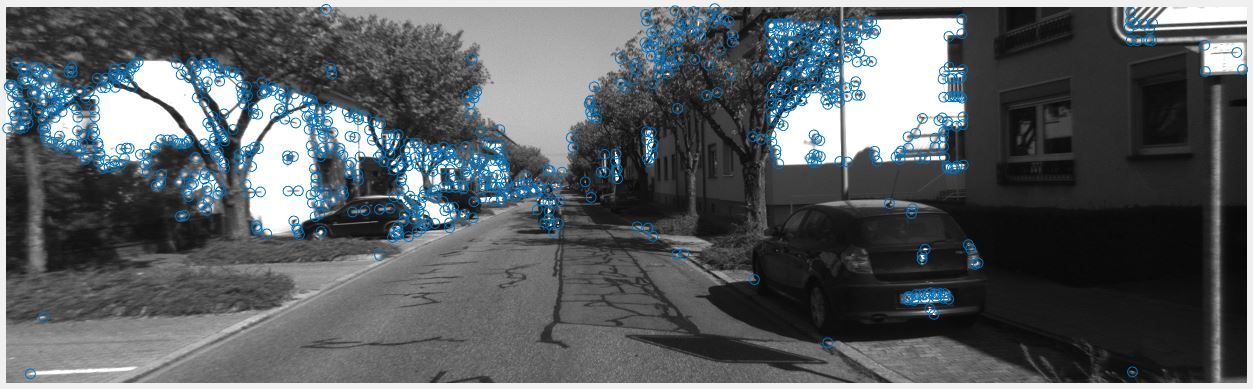
\includegraphics[width=0.7\linewidth]{Pictures/HarrisBad}

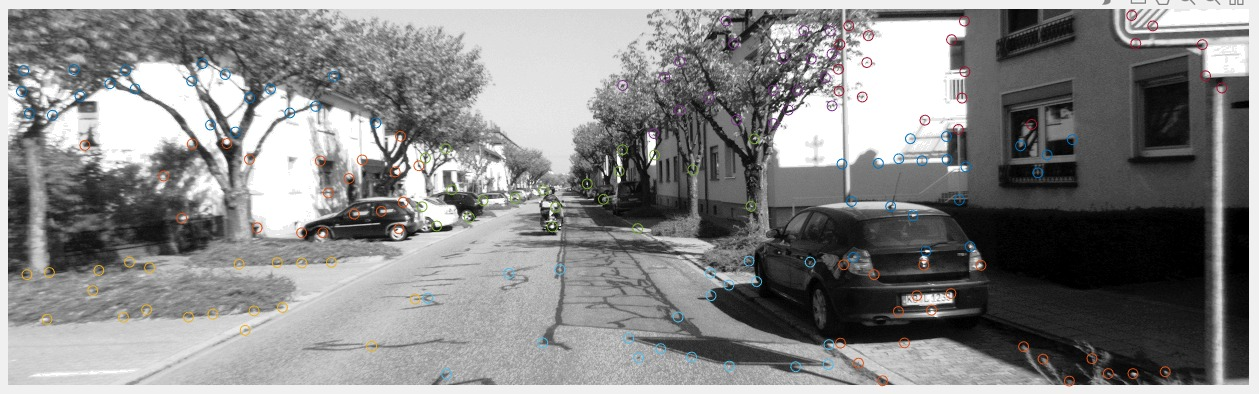
\includegraphics[width=0.7\linewidth]{Pictures/LocalizedHarrisGood}
\end{center}
\caption{Comparison of standard Harris (above) with the improved approach (below).}
\label{fig:HarrisVsHarris}
\end{figure}


\begin{algorithm}
\caption{Localized Harris Keypoints Non-Maxima Suppression}
\begin{algorithmic}[1]
\Function{loc\_harris\_nonmaxima\_sup}{\emph{grid,radius,npoints,minQuality,FilterSize}}
\State all\_points $\gets$ \{\}
\ForAll{cells \textbf{in} grid}
\State cell\_points $\gets$ detectHarrisFeatures(\emph{minQuality,FilterSize})
\While{number(filtered\_points) $<$ \emph{npoints}}\Comment{Point by point extraction}
\State filtered\_points $\gets$ NonMaximaSuppression(cell\_points, \emph{radius})
\EndWhile
\State all\_points $\gets$ filtered\_points
\EndFor
\EndFunction
\end{algorithmic}
\label{alg:LocHarr}
\end{algorithm}

\subsection{Horizontal Rotation Recovery \& Feature Removal}
\label{sec:yaw}
We encountered the problem in our own datasets that on a pure horizontal rotation (around the camera y-axis) of the camera many landmarks were lost, but no new features were added based on the angle threshold imposed on the promotion of candidates.
%
This happens since the bearing vectors are only changing in inertial frame when the camera undergoes a translational motion.
%
Without any translational motion no new landmarks are added based on the proposed bearing vector angle.
%
To solve the problem we introduced a second possibility for candidates to be promoted, which is based on the idea that candidates that have been tracked for a sufficient amount of frames must be somehow reliable.
%
Then among those a pixel threshold is imposed, which promotes candidates that have traveled at least a certain distance on their track.
%
The motivation behind this is that pixel who have moved enough through the frame without being promoted by the bearing vector angle, are likely points that are far away in relation to the movement of the camera.
%
Even if these points can not be triangulated  so reliably they still can be useful to estimate the rotation of the camera.

The problem introduced with this practice was a vast amount of new landmarks when performing a prolonged rotation. We recorded peaks of up to 6000 features. The solution was to set a limit of 500-1000 features. After that threshold is passed keypoints are removed  by choosing one after another and always eliminating all keypoints within a certain radius.

\subsection{Pose Refinement}

When localizing an new frame based on the tracked keypoints and on the current landmarks using P3P and subsequently DLT on the best inlier set, a small pose refinement is conducted. We minimize the reprojection error of all found inliers by optimizing the pose. Only very few iterations are necessary to reduce the reprojection error quiet a bit.

\subsection{Checking Reprojection Error of new Landmarks}

When assessing the validity of new landmarks, in addition to enforcing an angle threshold, the reprojection error of the candidate landmarks is limited as well. This is important since wrong feature tracks or moving scene objects can result in bearing vectors that are skew, and therefore do not intersect at all. In this case the triangulated landmark are not very helpful and should be omitted. Fortunately, this case can be captured very effectively by looking at the reprojection error of the landmark. Candidates with a large reprojection error are consequently removed from the state.

\subsection{Tunable Parameters}

\renewcommand{\arraystretch}{1.3}
\begin{TTable*}{llp{0.4\linewidth}@{\hskip 4ex}c}{Tunable Parameters}{Tunable Parameters}{tab:TunableParameters}
Functionality&Parameter Name&Description&Range\\\midrule
Harris&\texttt{rows}&Number of rows of the grid.&3 - 5\\
&\texttt{cols}&Number of columns of the grid.&3 - 5\\
&\texttt{radius}&Radius used for the non maxima suppression.&4 - 10\\
&\texttt{npoints}&Desired number of features per grid cell.&30 - 45\\
&\texttt{minQuality}&Minimum allowed quality for harris features.&0.01\\
&\texttt{FilterSize}&Gaussian filter dimension for detection of harris features.&3 - 25\\
Matching&\texttt{maxBidirectionalError}&Forward-backward error threshold for KLT tracking.&2.7 - 3\\
&\texttt{radius\_to\_new\_feature}&Minimum distance between existing features (keypoints and candidates) and new candidates.&2 - 5\\
&\texttt{KLT\_score\_limit}&Minimum quality of KLT tracked features.&0.997\\
&\texttt{block\_size}&Size of neighborhood around each point being tracked for KLT tracking.&25 - 35\\
Localization&\texttt{RANSAC\_iteration}&Number of performed RANSAC iterations.&1k - 3k\\
&\texttt{RANSAC\_error}&Maximum reprojection error for inliers.&3.5 - 10\\
Triangulation&\texttt{sanity\_check\_factor}&Determines depth after which landmarks are removed.&7\\
&\texttt{angle\_threshold}&Angle threshold for new landmarks.&1.5 - 5\\
&\texttt{age\_threshold}&Minimum track duration for a new candidate to be promoted to landmark.&8 - 10\\
&\texttt{pixel\_threshold}&Minimum pixel distance for a new candidate to be promoted to landmark.&35\\
BA&\texttt{periode}&Number of frames until next optimization.&5 - 10\\
&\texttt{window\_size}&Window size for windowed BA.&12 - 20\\
&\texttt{max\_iteration}&Maximum number of iterations for \texttt{lsqnonlin}.&15 - 20\\
\end{TTable*}

The feature detector's and tracker's parameter had to be well tuned for each single dataset. The tuning depends mostly on the image resolution and the image content and structure. Depending on how good the tracking works over the whole sequence one has to adapt the number of RANSAC iterations for the localization. Since it is not required to boost the efficiency of the code, the RANSAC iterations are chosen rather conservatively. The angle threshold for new landmarks had to be chosen rather small, such that we add new landmarks fast enough during corner turns.

\section{Milestones}

\renewcommand{\arraystretch}{1.3}
\begin{TTable*}{llllp{0.3\linewidth}}{Overview of Project Milestones}{Overview of Project Milestones}{tab:ProjectMilestones}
&Name&Task&Problems&Solutions\\\midrule
\texttt{1}&Setup&Problem identification&Complexity&Divide and conquer, functional programming, paper prototyping, skeleton main file with function prototypes\\
&&Team organisation&Communication&Regular meetings, teamchat\\
&&Code organisation&Collaboration&Git for code, \LaTeX\ for documentation\\
&&Data handling&Diversity&Establish dataset class equipped with methods for loading data, getting frames, loading tuning parameter.\\\midrule
\texttt{2}&Basics&Implement basic features&Conventions&Adhere to established conventions to improve readability and consistency.\\
&&Bootstrapping&Feature Integration&Clarify misconceptions\\\midrule
\texttt{3}&\multirow{3}{*}{\shortstack[l]{Minimum\\\vspace{0.3ex}\\Viable\\\vspace{0.3ex}\\Product}}&Continuous Operation&Overview&Code refactoring and reorganisation of the folder structure\\
&&&Small bugs&Peer review and debugging plots\\
&&Tuning&Poor Performance&Realizing that tuning the feature detector and the feature tracker is critical for the performance of the pipeline.\\\midrule
\texttt{4}&Extension&Produce Datasets&Calibration&Realize that calibration is specific to video format.\\
&&&Distortion&Only allow detection of features within the valid image region of the undistorted frame.\\
&&BA&Parse state history & Carefully associate keypoints with the right landmark.\\
&&& Poor performance & Fix first two poses.\\
\end{TTable*}
%Usage:
%\begin{TTable}[<startindex for colors>]
%{<table layout>}
%{<your short caption>}
%{<your caption>}
%{<your label>}
%<your Content>
%\end{TTable}
%Dependencies: \usepackage{booktabs,xcolors,xparse}

\subsection{Most Interesting Problems}

The most challenging problem was actually getting the pipeline to work after having established its basic functionality. We realized that debugging it as a whole is basically impossible and thus decided to split the work and reiterate on the building blocks. Mostly by improving the debugging plots we realized that we were only generating new landmarks that were extremely close the the position of the camera. Without useful new landmarks the localisation breaks down very fast even if the feature tracking works well. The problem was that checking whether the candidate keypoints have travelled a large enough angle and performing the sanity check was not a sufficient condition for valid new landmarks. Instead we decided to limit the reprojection error which was key for getting the VO pipeline to run reasonably.

\section{Results}

The following section will give critical information about the uploaded screencasts.
%
The different plots included in the screencast are explained in figure \ref{fig:screencast}.
%
The relevant screencasts were run on a machine with the following specs: $8\cdot\SI{2.5}{\giga\hertz}$ CPU, $\SI{8}{\giga\byte}$ RAM and using a maximum of 121 threads.
%
The videos are provided \href{https://www.youtube.com/watch?v=kb6LgC9SKW4&list=PLQ0WlGP2XqesJnw_vhn5eEh0ukmRttWWv&index=1}{here}.

\begin{figure}[h]
\begin{center}
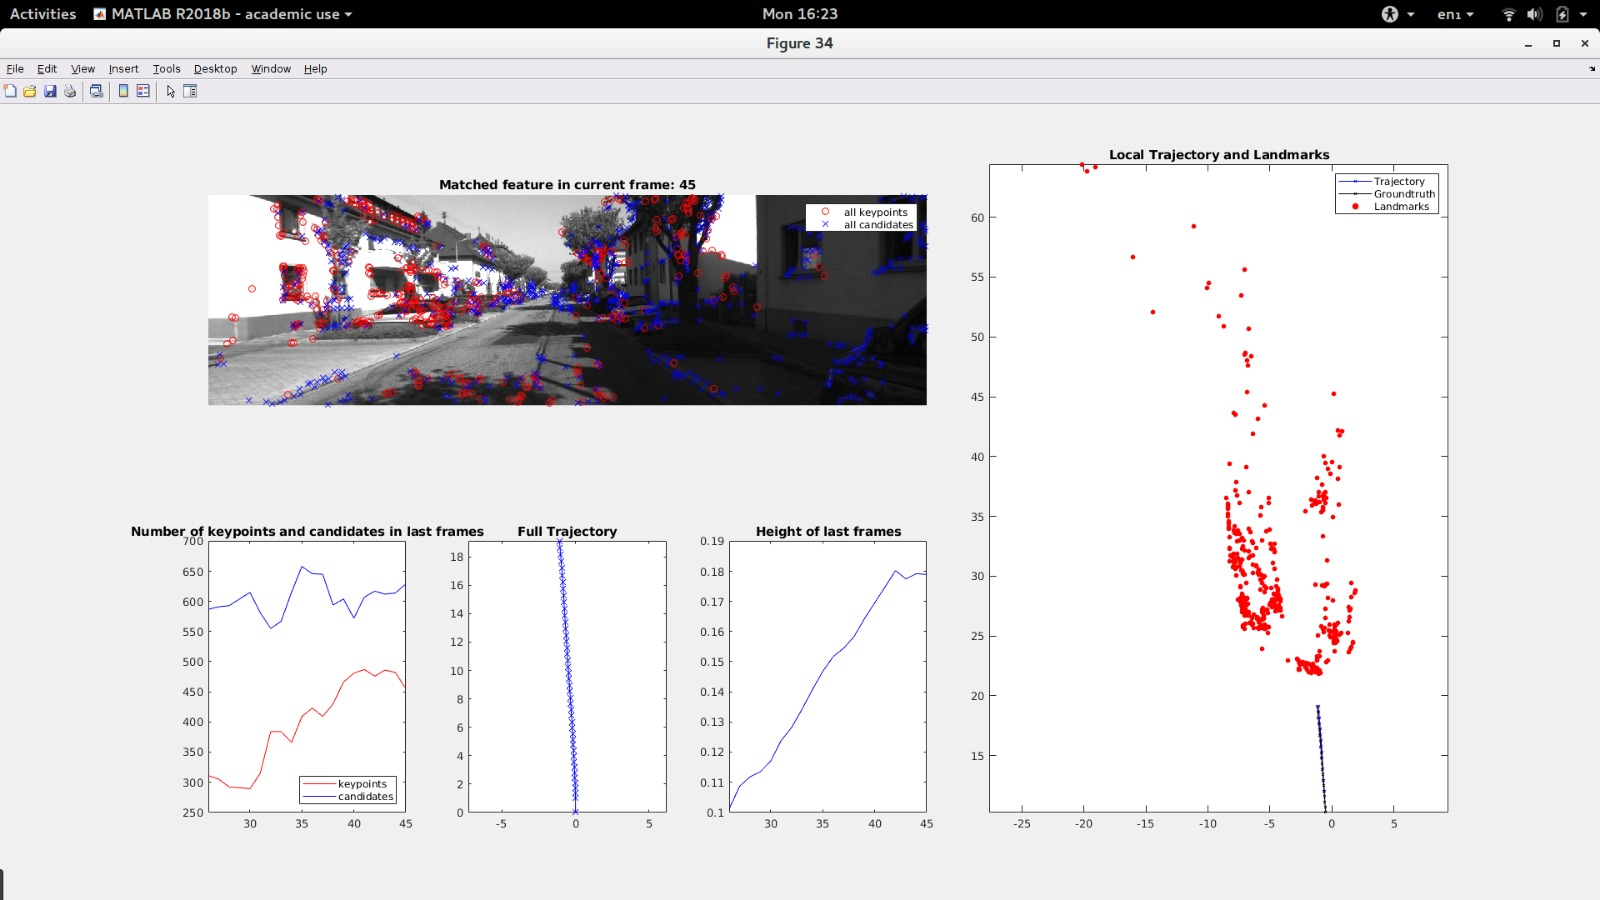
\includegraphics[width=\linewidth]{Pictures/Screencast}
\end{center}
\captionsetup{singlelinecheck=false}
\caption[Description of the Screencast]{The elements included in the screencast are, from top left to bottom right: The current frame with all current keypoints candidates, the number of keypoints vs. the number of candidates over time, the full trajectory either in 2D or in 3D, the height of the camera pose over time and the trajectory over the last few frames compared to ground truth and showing all current landmarks.}

\label{fig:screencast}
\end{figure}

To evaluate the pipeline, a qualitative comparison was made by adding the ground truth to the local plot.
%
The ground truth was transformed, such that the first pose of the last twenty frames align with the one of the generated trajectory.
%
Furthermore, the scale of the ground truth has been adapted to fit.
%
Hence, scale drifts are not that visible in this comparison.
%
However, the result of this comparison looks very promising.
%
The difference is only marginal.
%
Even when looking at the full trajectory of the kitti datset, the result seems to be plausible.

%
There were multiple things leading to an accurate trajectory.
%
The biggest impact came from the pose refinement and the bundle adjustment, which both improved the localization and triangulation significantly.
%
Next to that, the decision to split the image in multiple regions and search for key points in all of them individually helped to make the localization more robust.
%
Since we added multiple dataset with cameras on drones, we adapted are pipeline to be able to deal with fast yaw rotations without losing landmarks.
%

%
One of the actions of the pipeline is to remove all landmarks which are behind the camera.
%
This leads to a better localization, but can lead to a failing behavior.
%
If the localization determines (falsely) a large rotation, many landmarks will be removed, such that the pipeline could break.
%
To lower the risk of poor pose estimation and therby such actions, a high number of ransac iterations has been chosen.
%

\subsection{Parking}
The VO pipeline runs on the parking dataset very nicely. The feature tracking and the localization work very reliably. The performance increased quiet a lot by implementing a sliding window bundle adjustment as described in section \ref{sec:BA}.

\subsection{Kitti}
The results of the VO pipeline on the Kitti dataset are looking very promising. The overall trajectory looks quiet reasonable. A bit of slow scale drift is noticeable.
The dataset contains a few video sequences with high contrast scenes. In these sequences we had sometimes problems with the feature tracking. In these situation the localization lost its robustness. As already mentioned above a poor pose estimation can lead to the removal of almost all landmarks during the sanity check of the landmarks, which can break the VO pipeline. Due to this it was not possible to run the whole dataset at once without having to restart it a few frames before the break down.

\subsection{Malaga}
In our opinion this is the most difficult dataset to handle. It is very hard to tune the addition of new landmarks. On one side new landmarks should be added very quickly to deal with the sharp turn, on the other side landmarks should be added very conservatively to not get landmarks of detected features in the cloud and at borders of overexposed image regions. We think that this could have caused the rather large scale drift that we have experienced on this dataset.

%\small
%\renewcommand{\arraystretch}{1}
%\begin{TTableNonFloat*}{llllllll}
%Parameter Name&Kitty&Malaga&Parking&Bike&fpv1&fpv2&fpv3\\\midrule
%\texttt{rows}&4&4&3&4&4&4&4\\
%\texttt{cols}&5&5&3&4&5&5&5\\
%\texttt{radius}&4&4&6&10&4&4&4\\
%\texttt{npoints}&30&40&30&45&30&30&40\\
%\texttt{minQuality}&0.01&0.01&0.05&0.01&0.01&0.01&0.01\\
%\texttt{FilterSize}&5&25&11&3&15&5&5\\
%\texttt{maxBidirectionalError}&3&2.7&2.8&3&2.8&2.8&2.9\\
%\texttt{radius\_to\_new\_feature}&2&4&5&2&2&2&5\\
%\texttt{KLT\_score\_limit}&0.9965&0.997&0.996&0.9965&0.997&0.997&0.997\\
%\texttt{block\_size}&35&31&31&31&25&35&25\\
%\texttt{RANSAC\_iteration}&1500&3000&2000&1000&1000&1000&1000\\
%\texttt{RANSAC\_error}&4&3.5&8&10&5&5&5\\
%\texttt{sanity\_check\_factor}&7&7&7&7&7&7&7\\
%\texttt{angle\_threshold}&1.5&1.5&5&2&1.5&1.5&1.5\\
%\texttt{age\_threshold}&-&-&-&8&8&8&8\\
%\texttt{pixel\_threshold}&-&-&-&35&35&35&35\\
%\texttt{periode}&10&10&5&5&8&8&8\\
%\texttt{window\_size}&20&20&12&12&16&16&16\\
%\texttt{max\_iteration}&15&20&20&20&20&20&20\\
%\end{TTableNonFloat*}
%\normalsize
%The age and pixel threshold were not used for the following datasets: kitti, malaga, parking.

\subsection{Bike Zurich Straight}

This dataset shows a short bike ride along a straight street. It was recorded at high framerate and has a higher resolution than the provided datasets. Therefore a lot of harris corners can be detected and tracked reliably. Since we have chosen radius\_to\_new\_feature rather small, the number of tracked keypoints increases very fast. As soon as the number of keypoints are bigger than a certain threshold we remove to close keypoints from the state. This explains why the number of landmarks is changing a lot. This behavior can also be observed in the fpv dataset, which are described in the next section. A simple solution would be to increase the  radius\_to\_new\_feature, which would help to run the VO a bit faster.

\renewcommand{\arraystretch}{1.3}
\begin{TTableNonFloat*}{ll}
Location&Zurich\\
Motion&Handheld on a bike\\
Device&Gopro Hero 6 (no stabilization)\\
Resolution&1920x1080\\
Number of Frames& 1653\\
Framerate&120 fps (downsampled to 60 fps)\\
\end{TTableNonFloat*}

%\small
%\renewcommand{\arraystretch}{1}
%\begin{TTableNonFloat*}{ll}
%Parameter Name&Value\\\midrule
%\texttt{rows}&3\\
%\texttt{cols}&4\\
%\texttt{radius}&10\\
%\texttt{npoints}&45\\
%\texttt{minQuality}&0.01\\
%\texttt{FilterSize}&3\\
%\texttt{maxBidirectionalError}&3\\
%\texttt{radius\_to\_new\_feature}&2\\
%\texttt{KLT\_score\_limit}&0.9965\\
%\texttt{block\_size}&31\\
%\texttt{RANSAC\_iteration}&1000\\
%\texttt{RANSAC\_error}&10\\
%\texttt{sanity\_check\_factor}&7\\
%\texttt{angle\_threshold}&2\\
%\texttt{age\_threshold}&8\\
%\texttt{pixel\_threshold}&35\\
%\texttt{periode}&5\\
%\texttt{window\_size}&12\\
%\texttt{max\_iteration}&20\\
%\end{TTableNonFloat*}
%\normalsize

%\subsection{Bike Zurich} %Not tuned yet

%\subsection{Walk Indoor ETHZ} %Not tuned yet


\subsection{FPV 1,2,3}

Three datasets - FPV1, FPV2 and FPV3 - were recorded with a racing drone.
%
Therefore the camera is moving in all 6 DOF.
%
One challenge is the fast horizontal rotation that can occur even when the camera is staying at the same position.
%
As explained in section \ref{sec:yaw}, our VO pipeline also adds new landmarks in these situation.
%
This can be observed for example in the middle of the FPV1 dataset.
%
After a short rise, the drone performs a 180 degree yaw motion before it then dives down again.
%
Turning this yaw motion it only can track features that are relatively far away.
%
Even tough these potential landmark were always observed from the same point, we add them if they are tracked for a long enough duration and if they moved enough trough the image frame.
%
Since the triangulation of these landmarks includes a rather high uncertainty, small jumps in the camera poses can be observed during this turn.
%
Nevertheless the proposed solution manages to deal with these situation quiet well.

\renewcommand{\arraystretch}{1.3}
\begin{TTableNonFloat*}{ll}
Location&Schüpfheim, LU\\
Motion&Drone flight\\
Device&Gopro Hero 6 (no stabilization)\\
Resolution&1920x1080\\
Number of Frames& [706,1660,1412]\\
Framerate&60 fps (downsampled to 30 fps)\\
\end{TTableNonFloat*}


%\small
%\renewcommand{\arraystretch}{1}
%\begin{TTableNonFloat*}{ll}
%Parameter Name&Value\\\midrule
%\texttt{rows}&4\\
%\texttt{cols}&5\\
%\texttt{radius}&4\\
%\texttt{npoints}&30\\
%\texttt{minQuality}&0.01\\
%\texttt{FilterSize}&15\\
%\texttt{maxBidirectionalError}&2.8\\
%\texttt{radius\_to\_new\_feature}&2\\
%\texttt{KLT\_score\_limit}&0.997\\
%\texttt{block\_size}&25\\
%\texttt{RANSAC\_iteration}&1000\\
%\texttt{RANSAC\_error}&5\\
%\texttt{sanity\_check\_factor}&7\\
%\texttt{angle\_threshold}&1.5\\
%\texttt{age\_threshold}&8\\
%\texttt{pixel\_threshold}&35\\
%\texttt{periode}&8\\
%\texttt{window\_size}&16\\
%\texttt{max\_iteration}&20\\
%\end{TTableNonFloat*}
%\normalsize


\section{Additional Features}

\subsection{Datasets}

As an additional feature a series of datasets was recorded.

\begin{enumerate}
\item \textbf{Camera calibration}

% I think we can let this be.
%\begin{figure}[b]
%\sbss{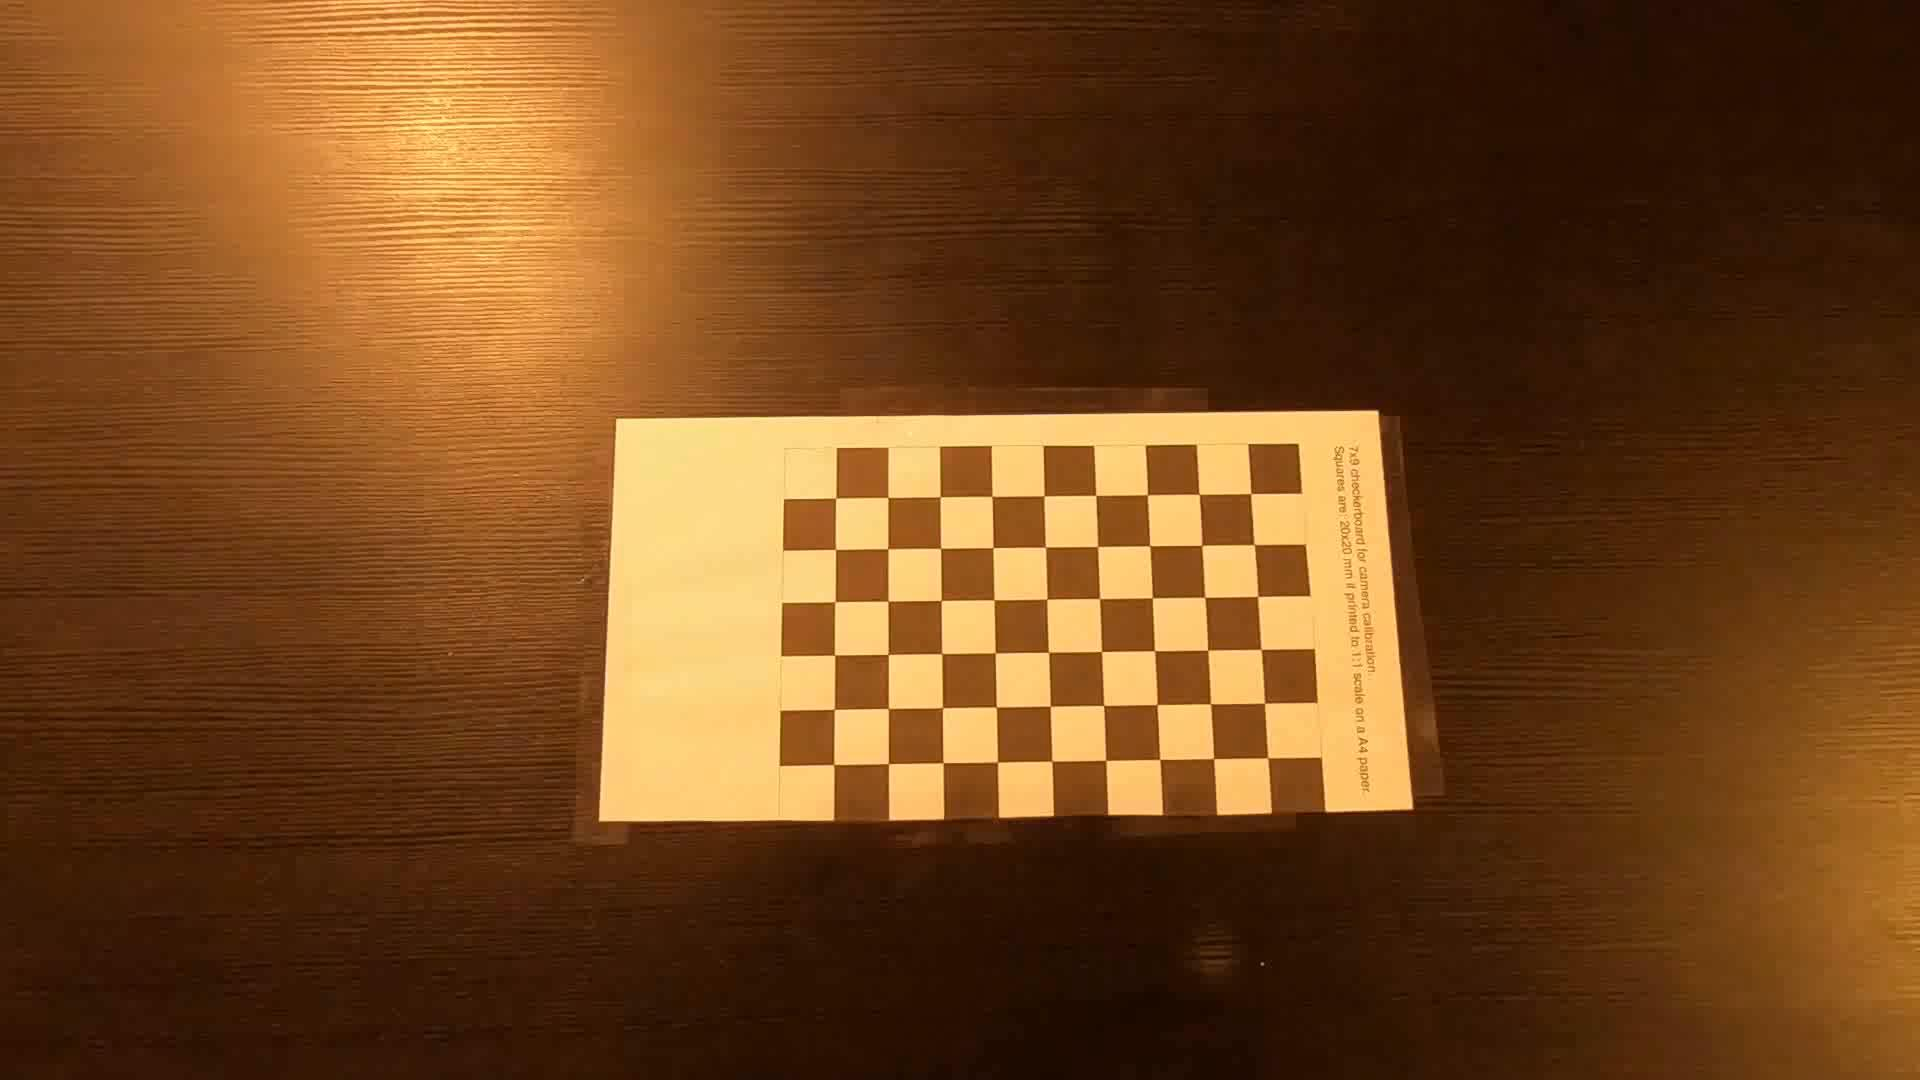
\includegraphics[width=\linewidth]{Pictures/CalibrationGoPro}}{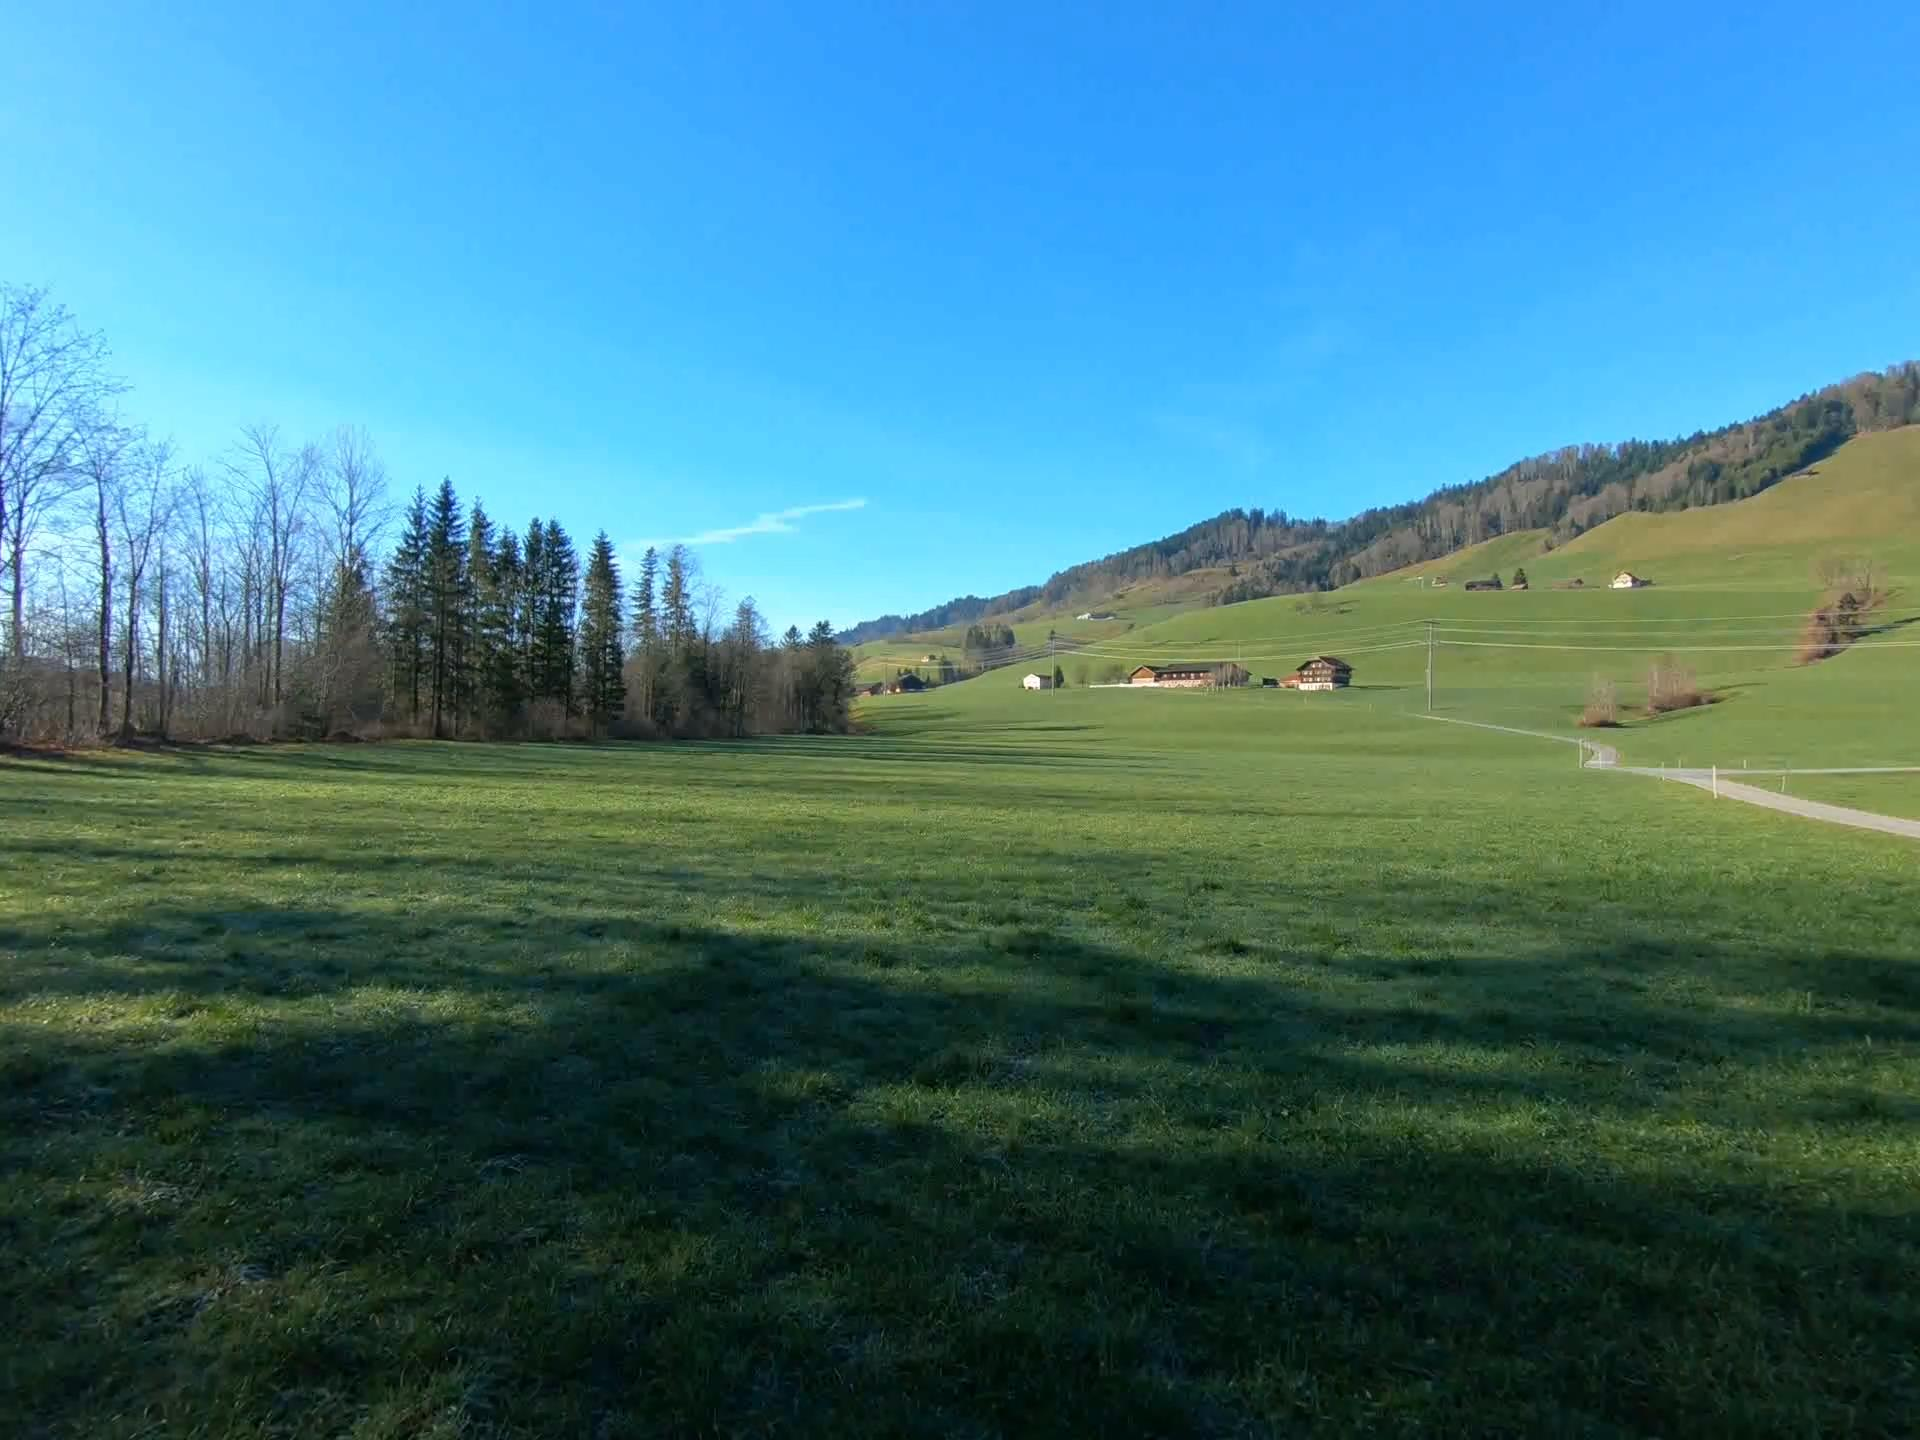
\includegraphics[width=\linewidth]{Pictures/ImageGoPro}}
%\caption{Left: Frame of the calibration video, right: frame of the dataset}
%\label{fig:fpv1}
%\end{figure}

The Gopro 6 was calibrated based on a short clip of a checkerboard, using the calibration toolbox in Matlab. The size of the used checkerboard, on A4 paper, is rather small. Therefore the checkerboard has to be held rather close in front of the camera. This could decrease the quality of the calibration. Nevertheless, a very nice performance on our custom datasets could be observed.  Another issue arose after undistorting the images which led to black padding around the image. In order to avoid to crop the image, harris corners at the border of the frame are discarded.

\item \textbf{Dataset}
A first test dataset was recorded handheld on a bike. To create a more interesting dataset, the camera was mounted on a racing drone. This makes for various camera motions like rolling and pitching. Even though the motion was rather fast the high frame rate of 60 fps and thus short exposure made for sharp images. For reducing computational effort every second image was used, reducing the effective frame rate by half.
\end{enumerate}

\subsection{Sliding Window Bundle Adjustment}
\label{sec:BA}
For refinement of the trajectory bundle adjustment was implemented.
%
To reduce the cycle time the implementation proposed in exercise 9 was extended with a sliding window, therefore only optimising a certain number of past frames.
%
The implementation includes the precalculation of the jacobian's non-zero elements to maximize speed.

The extraction of landmarks from the state history, the mapping to the corresponding landmarks and the restructuring for the optimization framework was challenging.
%
First we assume that landmarks have the same coordinates throughout the considered window.
%
By this we find correspondences between the different frames.
%
Then we use Matlab's \verb+unique+ to find the unique set of landmarks viewed during the chosen track.
%
Finally this set is restructured to fit the data structure given in exercise 9.

To make sliding window bundle adjustment effective, a measure for connecting the independently optimized piece of the trajectory to its past has to be found.
%
The approach proposed is to introduce continuity constraints by explicitly excluding the first two poses of the current segment from the optimization.
%
Continuity is  enforced by still optimizing the reprojection error of the landmarks in the two poses.
%
This solution effectively keeps the trajectory smooth.
%
In order to not change the scale during the bundle adjustment also the second pose of the window is kept constant.
%
The window size and periode are chosen such that the first two frames of the window are already optimized in the previous iteration.


To see how much the bundle adjustment improves the performance of the VO pipeline, a test case was set up on the parking dataset.
%
In this test we compare the trajectory with and without bundles adjustment to the ground truth.
%
To get the scale of the monocular VO right, the pose of the ground truth was used for the bootstrapping.
%
Landmarks with a big reprojection error are removed to get a good bootstrapping.
%
Five runs of the VO pipeline were performed with and without bundle adjustment with the same bootstrapping and then compared to the ground truth trajectory.
%
The following error measurement was used to determine the performance of the trajectory

\newcommand{\norm}[1]{\left\lVert#1\right\rVert_2}
$$\sum_i \norm{s_i \cdot t_{i,i+1}^{vo} - t_{i,i+1}^{gt}} \text{\qquad ,where \quad} s_i = \tfrac{\norm{t_{i-1,i}^{gt}}}{\norm{t_{i-1,i}^{vo}}} $$

, where $t_{i,i+1}^{vo}$ is the translation vector from camera pose $i$ to camera pose $i+1$ of the VO trajectory.
%
$t_{i,i+1}^{gt}$ is the translation vector between camera poses of the ground truth trajectory.
%
The scale factor $s_i$ is used in the error equation to compensate for the scale drift that occurred in previous frames.
%
Since this error measurement is looking at the error from frame to frame, and not only comparing the last poses of both trajectories, it is not so sensitive to rotation errors and scale drifts in the beginning of the trajectory.

The VO pipeline without bundle adjustment showed a mean error of 5.548 and a standard deviation of 0.505, while the VO pipeline with bundle adjustment showed a mean error of 1.597 and a standard deviation of 0.008.
%
The bundle adjustment seems not only improve the performance of the VO pipeline, but also to make it performance more consistent.

\end{document}
